\chapter{Los registros existentes}
\addcontentsline{toc}{chapter}{Los registros existentes}

En el laboratorio remoto se ha registrado la actividad de $7$ años consecutivos (desde el curso académico $1516$ al $2122$). Un ejemplo de las interacciones almacenadas puede verse en la Tabla \ref{tab:example}.

\begin{table}[H]
\centering
\caption{Muestra de los datos que se recopilan en el servidor.}
\label{tab:example}
\begin{tabular}{cccccc}
\hline
\textbf{Year} & \textbf{Group} & \textbf{SessionID} & \textbf{Date}       & \textbf{Problem} & \textbf{Step} \\ \hline
1819          & Keid           & 493252533735       & 28/10/2018 20:23:35 & P1               & 1             \\ 
1819          & Keid           & 493252533735       & 28/10/2018 20:23:40 & P1               & 3             \\ 
1819          & Keid           & 389034076811       & 7/11/2018 19:01:49  & P2               & 1             \\
1819          & Cerastes       & 487544594557       & 27/10/2018 13:05:11 & P1               & 1             \\
1819          & Cerastes       & 487544594557       & 27/10/2018 13:10:57 & P1               & 3             \\
1819          & Jabbah         & 550676318711       & 20/12/2018 22:22:42 & P8               & 1             \\
1819          & Cerastes       & 336303012053       & 17/12/2018 13:28:50 & P9               & 1             \\ 
1819          & Keid           & 563159878397       & 25/10/2018 12:41:43 & P8               & 1             \\ \hline
\end{tabular}
\end{table}

\section{Número de grupos cada año}

El número de grupos puede variar en cada curso en función del número de alumnos matriculados en la asignatura ese año. Así pues, se muestran a continuación en las Tablas \ref{tab:groups1} y \ref{tab:groups2} los grupos por curso académico.

\section{El periodo de tiempo analizado cada año}

En la Tabla \ref{tab:days} se muestra el número de días que dura la práctica cada año. Se puede apreciar que la duración de la práctica que estamos considerando puede variar en función del curso académico.

\begin{table}[H]
\centering
\caption{Número de días que dura la práctica cada año.}
\label{tab:days}
\begin{tabular}{cc}
\hline
\textbf{Year}  & \textbf{Length (days)}  \\ \hline
Y2015 & 33 \\
Y2016 & 24 \\
Y2017 & 30 \\
Y2018 & 18 \\
Y2019 & 28 \\
Y2020 & 17 \\
Y2021 & 39 \\ \hline
\end{tabular}
\end{table}

\section{El conjunto de problemas analizados cada año}

Todos los años hay 9 problemas de dificultad similar que deben ser resueltos por todos los grupos.

Para aproximarnos al concepto subjetivo de ``dificultad del problema'' vamos a analizar el número de sesiones fallidas que necesita cada alumno para resolverlos por primera vez con respecto al número total de sesiones de ese problema (tasa de fallo) y la duración de este periodo en horas.

\subsection{Dificultad del problema: la tasa de fallo}

La apertura de un problema se corresponde con una sesión de trabajo, la cual puede terminar como fallo (fail) si no se consigue resolver el problema, o éxito (solved) en caso de que se haya resuelto el problema. Así pues, se definirá la tasa de fallo como el cociente entre el número total de sesiones fallidas entre el número total de sesiones de un mismo problema. El boxplot de las tasas de fallo por problema puede verse en la Figura \ref{fig:boxplotfailratio}.

\begin{figure}[H]
    \centering
    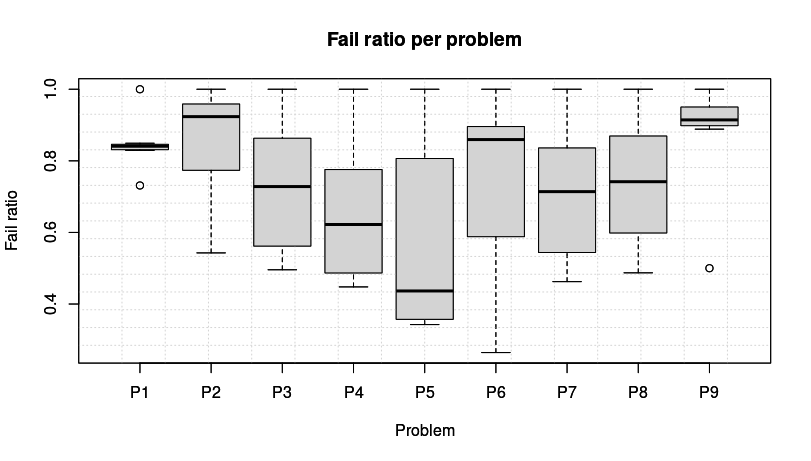
\includegraphics[width=0.85\textwidth]{Rplot09.png}
    \caption{Boxplot de la tasa de fallo (Fail ratio) por problema.}
    \label{fig:boxplotfailratio}
\end{figure}

Tras realizar el test ANOVA de un factor (resultados en la Tabla \ref{tab:ANOVAfailratio}), cuya hipótesis nula establece que la tasa de fallo media de los nueve problemas considerados es la misma, se detecta que las distribuciones de probabilidad de la tasa de fallo son estadísticamente iguales en los distintos problemas ($p = 0.1733 > 0.05$)\footnote{Nótese que hemos establecido un nivel de significancia de $\alpha = 0.05$.}.

% latex table generated in R 4.3.0 by xtable 1.8-4 package
% Sat May 27 20:17:56 2023
\begin{table}[H]
\centering
\caption{Resultados del test ANOVA de un solo factor (tasa de fallo).}
\label{tab:ANOVAfailratio}
\begin{tabular}{lrrrrr}
  \hline
 & Df & Sum Sq & Mean Sq & F value & Pr($>$F) \\ 
  \hline
ndsp[[nVariable]] & 8 & 0.51 & 0.06 & 1.52 & 0.1733 \\ 
  Residuals         & 54 & 2.26 & 0.04 &  &  \\ 
   \hline
\end{tabular}
\end{table}

Además, se ha realizado un test de Tukey por pares de problemas (Tabla \ref{tab:Tukeyfailratio}). En él se observa que casi todos los pares pueden considerarse estadísticamente iguales ($\text{p adj} > 0.2$ en todos ellos) salvo quizá, el par P9-P5 ($\text{p adj} = 0.2$). La Figura \ref{fig:confidenceratiofail} muestra los intervalos de confianza de todas las diferencias entre las distintas parejas de años.

\begin{figure}[H]
    \centering
    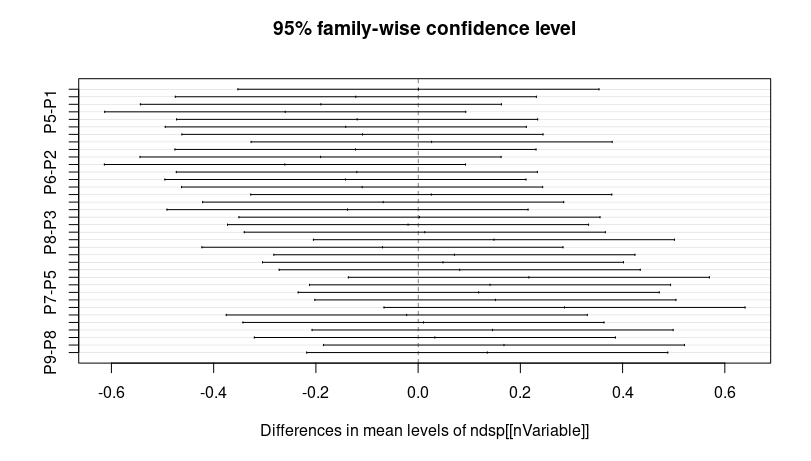
\includegraphics[width=0.80\textwidth]{Rplot10.png}
    \caption{Intervalos de confianza de la tasas de fallo de los problemas.}
    \label{fig:confidenceratiofail}
\end{figure}

%Estos datos hay que interpretarlos de manera incremental, pues para resolver un problema Pi requiere las habilidades de Pj(0<=j<i) más habilidades nuevas propias de Pi Periódicamente se incrementa notablemente el nivel de dificultad. P1 es el que más cuesta porque siempre cuesta trabajo empezar, P2-4 son muy parecidos y P5 es un poco más difícil, P6-P8 suben un escalón de dificultad y P9 también.

\subsection{Dificultad del problema: tiempo necesario en resolverlo}

Es el número de horas que transcurren desde que el problema se abre por primera vez hasta que es resuelto por primera vez.

\textbf{Falta imagen.}

De nuevo los tests detectan comportamientos diferentes (ANOVA p=9.27e-5, KW p=8.8e-8).

\textbf{Falta tabla.}

Por pares.

\textbf{Falta tabla.}

Intervalos de confianza.

\textbf{Falta imagen.}

Por lo tanto, se puede ver, dadas las evidencias aportadas que la resolución de cada problema exige respuestas claramente diferentes por parte del alumnado.

\section{Actividad registrada}\label{sec:activityrecorded}

El número de registros y de sesiones de trabajo de cada uno de los años analizados se muestran en la Tabla \ref{tab:records}. Como podemos ver, aunque el curso académico $2021$ registra más actividad que los demás, no es el que presenta un mayor número de sesiones.

\begin{table}[H]
\centering
\caption{Número de registros y sesiones almacenados en el servidor por años.}
\label{tab:records}
\begin{tabular}{ccc}
\hline
\textbf{Year}  & \textbf{Activity Records} & \textbf{Sessions}  \\ \hline
Y2015 & 12088            &  4489  \\
Y2016 & 12525            &  4538  \\
Y2017 & 9088             &  3661  \\
Y2018 & 5705             &  2811  \\
Y2019 & 14475            &  5156  \\
Y2020 & 21188            &  3900  \\
Y2021 & 11961            &  6113  \\ \hline
\end{tabular}
\end{table}

Al ser un servicio 24 horas los 7 días de la semana, los alumnos interactúan con el laboratorio remoto en cualquier día de la semana tal y como puede verse en la Figura \ref{fig:days} y a cualquier hora del día (Figura \ref{fig:hours}).

\begin{figure}[H]
\centering
\subfloat[Histograma de los días de la semana.]{\label{fig:days}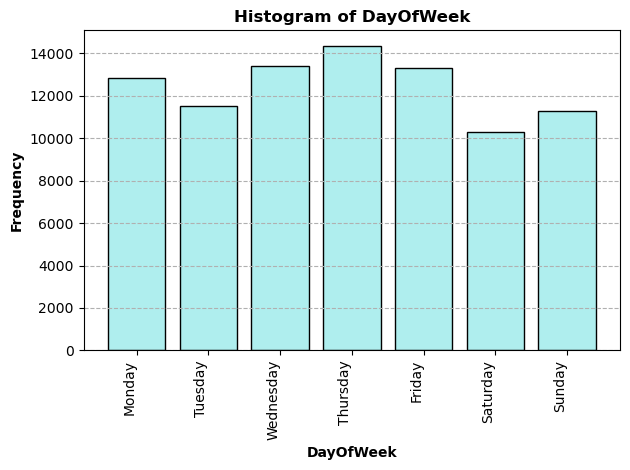
\includegraphics[width=0.47\textwidth]{histogramdayofweek.png}}\qquad
\subfloat[Histograma de las horas del día.]{\label{fig:hours}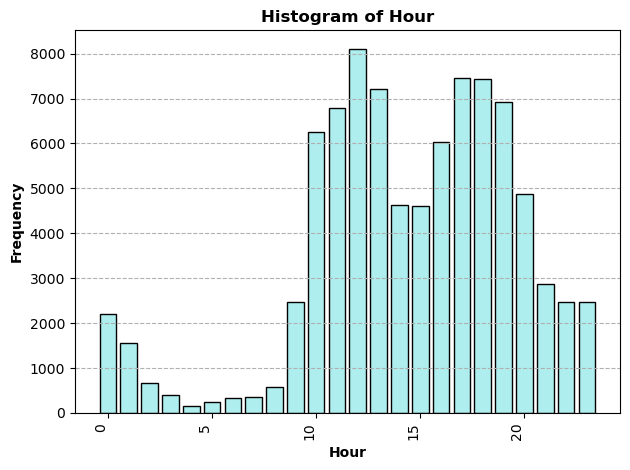
\includegraphics[width=0.47\textwidth]{histogramhour.png}}
\caption{Actividad registrada en el servidor remoto.}
\label{fig:activity}
\end{figure}

El número y tipo de las sesiones de trabajo de cada uno de los grupos puede contemplarse en la Tabla \ref{tab:type}.

\subsection{Análisis de la normalidad de la distribución del número de sesiones}

En las Figuras \ref{fig:boxplotresiduals} y \ref{fig:histogramresiduals} podemos ver el boxplot de los residuos y el histograma de los mismos.

\begin{figure}[H]
\centering
\subfloat[Boxplot de los residuos del número de sesiones.]{\label{fig:boxplotresiduals}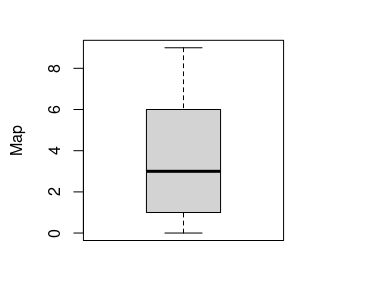
\includegraphics[width=0.47\textwidth]{Rplot02.png}}\qquad
\subfloat[Histograma de los residuos del número de sesiones.]{\label{fig:histogramresiduals}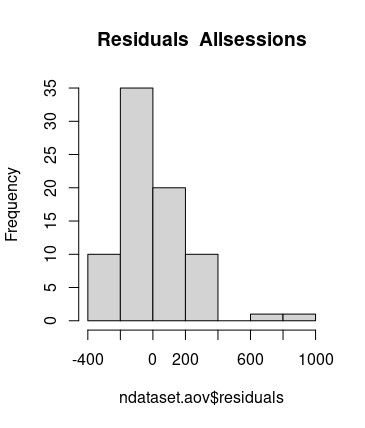
\includegraphics[width=0.47\textwidth]{Rplot03.png}}
\caption{Distribución de los residuos del número de sesiones.}
\label{fig:activity}
\end{figure}

A continuación, en las Figuras \ref{fig:densitysessions} y \ref{fig:q-qsessions}, podemos observar que la distribución del número de sesiones no es perfectamente normal pero es casi-normal si eliminaremos algunos outsiders.

\begin{figure}[H]
    \centering
    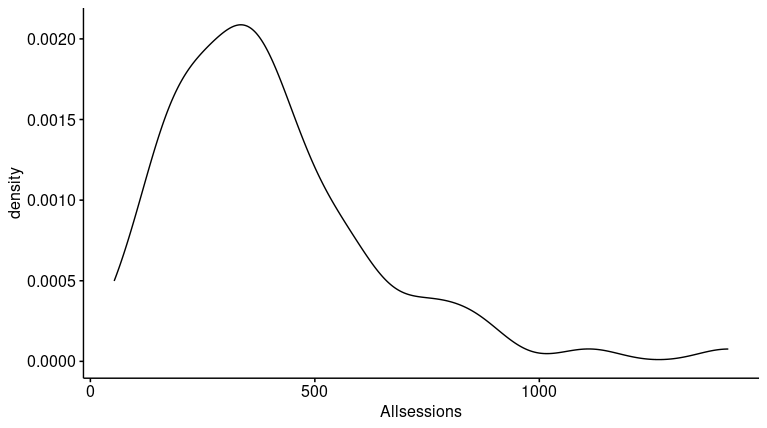
\includegraphics[width=0.75\textwidth]{Rplot04.png}
    \caption{Función de densidad de probabilidad del número de sesiones.}
    \label{fig:densitysessions}
\end{figure}


\begin{figure}[H]
    \centering
    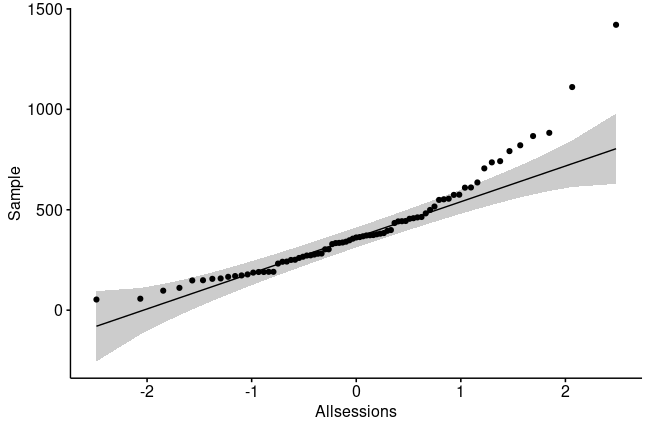
\includegraphics[width=0.75\textwidth]{Rplot05.png}
    \caption{Gráfico Q-Q del número de sesiones.}
    \label{fig:q-qsessions}
\end{figure}

\subsection{Sesiones por cada problema}

En la Figura \ref{fig:boxplotsessionsproblem} podemos ver el boxplot del número de sesiones por problema. Como podemos ver, el problema P1 es mucho más frecuentado que el resto. No obstante, esto se debe la principal diferencia entre el número de sesiones abiertas del problema P1 y restantes se debe a que los alumnos utilizan el primer problema como base de todos los experimentos y para testear las comunicaciones con el servidor. Así pues, el problema P1 es frecuentemente utilizado, no ya sólo al comienzo, sino durante toda la práctica.

\begin{figure}[H]
    \centering
    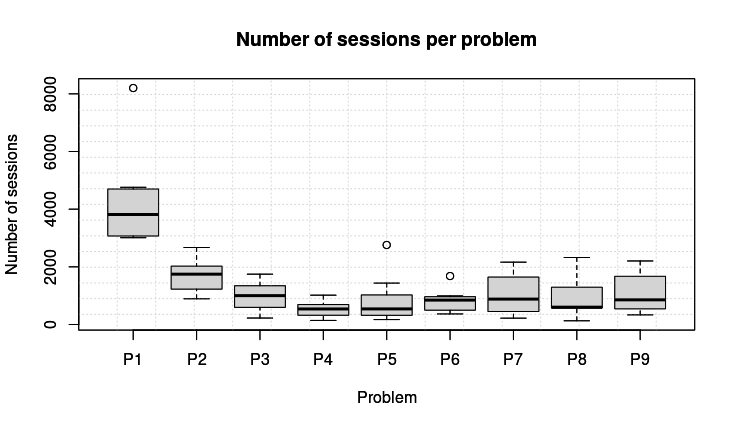
\includegraphics[width=0.85\textwidth]{Rplot06.png}
    \caption{Boxplot del número de sesiones por problema.}
    \label{fig:boxplotsessionsproblem}
\end{figure}

\subsection{Sesiones cada año}

Como podemos ver en la Figura \ref{fig:boxplotsessionsyear}, las sesiones de trabajo abiertas en el servidor año tras año, parecen seguir la misma distribución de probabilidad.

\begin{figure}[H]
    \centering
    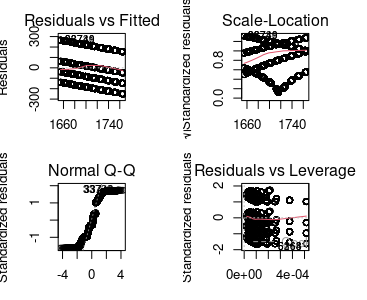
\includegraphics[width=0.80\textwidth]{Rplot07.png}
    \caption{Boxplot del número de sesiones por año.}
    \label{fig:boxplotsessionsyear}
\end{figure}

Un resumen de los resultados obtenidos al realizar el test ANOVA se muestra en la Tabla \ref{tab:ANOVAnumsessions}. La hipótesis nula establece que el número de sesiones medio de los siete cursos académicos estudiados es el mismo. Así pues, estableciendo un nivel de significancia de $0.05$, como tenemos que $p = 0.0630 > 0.05$, las diferencias entre las medias no son estadísticamente significativas.

% latex table generated in R 4.3.0 by xtable 1.8-4 package
% Sat May 27 18:26:28 2023
\begin{table}[H]
\centering
\caption{Resultados del test ANOVA de un solo factor (número de sesiones).}
\label{tab:ANOVAnumsessions}
\begin{tabular}{lrrrrr}
  \hline
 & Df & Sum Sq & Mean Sq & F value & Pr($>$F) \\ 
  \hline
ndsp[[nVariable]] & 6 & 666498.27 & 111083.05 & 2.11 & 0.0630 \\ 
  Residuals         & 70 & 3688035.44 & 52686.22 &  &  \\ 
   \hline
\end{tabular}
\end{table}

Además, se ha realizado un test de Tukey por pares de años (Tabla \ref{tab:Tukeynumsessions}). En él se observa que todos los pares pueden considerarse estadísticamente iguales ($\text{p adj} > 0.2$ en todos ellos). La Figura \ref{fig:confidencenumsessions} muestra los intervalos de confianza de todas las diferencias entre las distintas parejas de años.

% latex table generated in R 4.3.0 by xtable 1.8-4 package
% Sat May 27 18:26:44 2023
\begin{table}[ht]
\centering
\caption{Test HSD de Tukey (Honestly-significance-difference) del número de sesiones por año.}
\label{tab:Tukeynumsessions}
\begin{tabular}{rrrrr}
  \hline
 & diff & lwr & upr & p adj \\ 
  \hline
Y2016-Y2015 & 5.44 & -323.03 & 333.92 & 1.00 \\ 
  Y2017-Y2015 & 24.22 & -326.93 & 375.38 & 1.00 \\ 
  Y2018-Y2015 & -243.23 & -556.42 & 69.96 & 0.23 \\ 
  Y2019-Y2015 & -69.11 & -376.37 & 238.15 & 0.99 \\ 
  Y2020-Y2015 & -198.78 & -500.93 & 103.38 & 0.43 \\ 
  Y2021-Y2015 & -116.72 & -407.05 & 173.62 & 0.88 \\ 
  Y2017-Y2016 & 18.78 & -332.38 & 369.93 & 1.00 \\ 
  Y2018-Y2016 & -248.68 & -561.87 & 64.51 & 0.21 \\ 
  Y2019-Y2016 & -74.56 & -381.82 & 232.71 & 0.99 \\ 
  Y2020-Y2016 & -204.22 & -506.38 & 97.93 & 0.39 \\ 
  Y2021-Y2016 & -122.16 & -412.49 & 168.18 & 0.86 \\ 
  Y2018-Y2017 & -267.45 & -604.35 & 69.45 & 0.21 \\ 
  Y2019-Y2017 & -93.33 & -424.73 & 238.06 & 0.98 \\ 
  Y2020-Y2017 & -223.00 & -549.67 & 103.67 & 0.38 \\ 
  Y2021-Y2017 & -140.94 & -456.70 & 174.83 & 0.82 \\ 
  Y2019-Y2018 & 174.12 & -116.74 & 464.98 & 0.54 \\ 
  Y2020-Y2018 & 44.45 & -241.01 & 329.92 & 1.00 \\ 
  Y2021-Y2018 & 126.52 & -146.40 & 399.44 & 0.80 \\ 
  Y2020-Y2019 & -129.67 & -408.61 & 149.28 & 0.79 \\ 
  Y2021-Y2019 & -47.60 & -313.70 & 218.49 & 1.00 \\ 
  Y2021-Y2020 & 82.06 & -178.12 & 342.24 & 0.96 \\ 
   \hline
\end{tabular}
\end{table}

\begin{figure}[H]
    \centering
    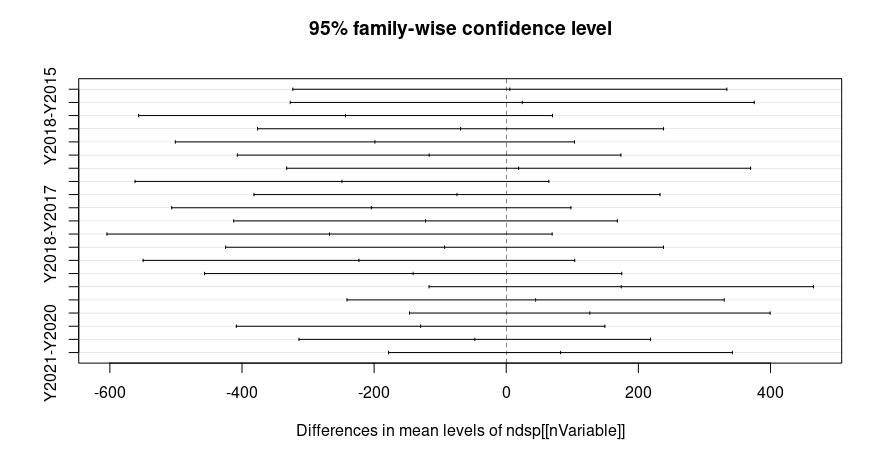
\includegraphics[width=0.80\textwidth]{Rplot08.png}
    \caption{Intervalos de confianza del número de sesiones por año.}
    \label{fig:confidencenumsessions}
\end{figure}